\section[时间]{\makebox[5em][s]{时间}}\label{sec:01.01}

描写物体的运动,要用时间和空间这两个概念。因此,我们
先来对时间、空间本身作一些分析。

时间和空间可以说是最平凡的概念了,因为在日常生活中也
常常用到它们。不过,若问什么是时间?什么是空间?却又不容易
找到恰当的答案。其实,这是两个很难的问题。尽管有不少关于
时间和空间的定义,但大都不能令人满意。一种或许可以接受的
说法是:时间、空间是物理事件之间的一种次序,时间用以表述
事物之同的顺序,空间用以表述事件相互之间的位形。

没有满意的“严格”的理论定义,并不妨碍时间和空间二者
在物理中的使用。因为,物理学是一门基于实验的科学,在考查
物理学的概念或物理量的时候,首先应当注意它与实验之间是否
有明确的、不含糊的关系。对于时间和空间这两个基本概念来说,
首要的问题似不是去追究它们的“纯粹”定义,而是应当了解它
们是怎样量度的。

量度时间,通常是用钟和表。然而,钟和表并不是测量时间
的唯一的工具。原则上。任何具有重复性的过程或现象,都可以
作为测量时间的一种钟。自然界里有许多重复性的过程,其中有
一些我们早已把它们当作计时标准了。例如,太阳的升没表示天;
四季的循环称作年;月亮的盈亏是农历的月。其他的循环过程,
如双星的旋转、人体的脉搏、吊灯的摆动,分子的振动等等,也
都可以用作测时的工具。

更一般地说,只要知道了某个物理现象随时间的变化,尽管
它不是重复性的过程,也可以用来测定时间。譬如,我们能从一
个人的容貌估计出他的年龄,因为容貌这个量与时间之间有确定
的关系。这个例子虽然很普通,但某些有用的测时方法与此是很
相似的。在确定星体的年龄时,常常就是根据星体的颜色。

钟的种类很多,但有好有坏。比较两个人的脉搏,就会发现
它们之间经常有明显的快慢波动,所以,人的脉搏不是一种好钟,
它不够稳定。如果比较一下两个单摆的周期,就会发现它们稳定
多了。地球自转则是更稳定的钟。
\begin{figure}[!h]
  \centering
  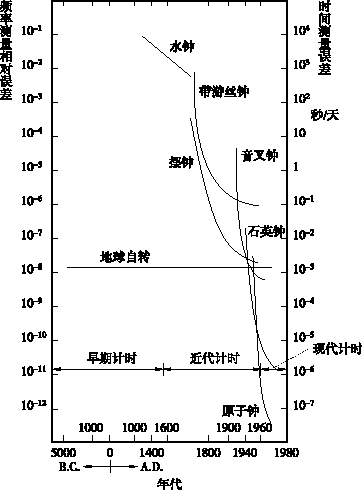
\includegraphics[height=8cm]{figure/fig01.01}
  \caption{不同年代的时间测量精度}\label{fig:01.01}
\end{figure}

\clearpage
图\ref{fig:01.01}给出不同年代用不同的钟测量时间所达到的精度。可以
看到,地球自转要比各种机械的钟都好。所以,1967年以前是用
地球自转作为标准钟。原子钟是比地球自转更加稳定的钟,现代
的精密计时都是用原子钟了。

\begin{table}[!h]
  \centering
  \caption{一些典型物理现象的时间尺度}\label{tab:01.01}
  \begin{tabular}{c}
    \toprule
    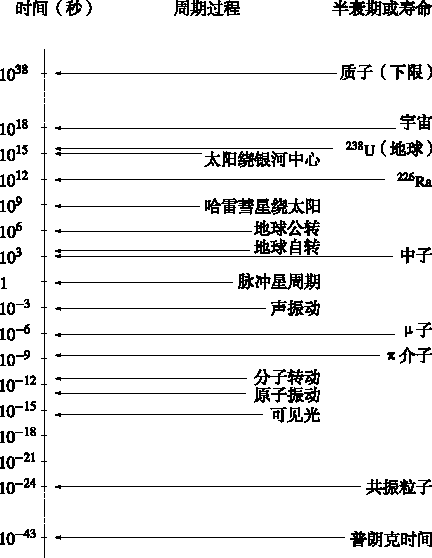
\includegraphics[width=0.8\linewidth]{figure/tab01.01} \\
    \bottomrule
  \end{tabular}
\end{table}
\clearpage
1967年10月在第十三届国际度量衡会议上通过了新的标准
钟,它对一秒的时间作如下的规定;位于海平面上的$^{133}$Cs原子
的基态的两个超精细能级在零磁场中跃迁辐射的周期$T$与$ 1 $秒的
关系为
\begin{equation*}
  1 \,\text{秒} = 9,192,631,770\,T
\end{equation*}

表\ref{tab:01.01}~列举了一些典型现象的时间尺度。目前,物理学中涉及
的最长的时间是:\num{e38}秒,它是质子寿命的下限。宇宙的年龄大约
是 \num{6e17}秒,即$ 200 $亿年。牛顿力学所涉及的时间尺度大约是
\num{e-3}$\sim$\num{e15}秒,即从声振动的周期到太阳绕银河中心转动的周期。
粒子物理的时间尺度都很小。$\mu$子的寿命是 \num{2e-6} 秒。已经算是
极长寿的了。最短寿的是一些共振粒子,它们的寿命只约有 \num{e-24}
秒。目前物理学中涉及的最小的时间是 \num{e-42}秒,称为普朗克时
间。普朗克时间被认为是最小的时间,比普朗克时间还要小的范
围内,时间的概念可能就不再适用了。
